\chapter{植物的无性繁殖与克隆}\label{ch:b2:asexual-reproduction}

犹他州某山谷中，矗立着一片由四万七千根白杨树干
组成的森林，实则只是一株植物：每根树干都由同一个根系
长出，每个细胞都携带相同的基因组，整个个体
约一万四千岁，重六千吨。
超市里同一品种草莓盒中的每一颗草莓，
都是同一株植物借匍匐茎繁殖出的一部分；地球上每一根卡文迪什香蕉
是同一株植物的\omterm{prop:b2:asexual-reproduction:horticulture}{扦插}苗的\omterm{prop:b2:asexual-reproduction:horticulture}{扦插}苗。与多数动物不同，植物
无需有性过程即可产生新个体——从一段茎、一条根、一片叶，
甚至烧瓶里的一个单细胞开始。本章讨论植物如何做到这一点、
园艺工作者如何利用这一能力，以及一个谱系放弃\omterm{def:b2:meiosis-heredity:meiosis}{减数分裂}和受精需付出什么代价，
即有性生殖为何存在这一根本问题。

\section{营养增殖}

\begin{definition}[克隆、基株、分株]\label{def:b2:asexual-reproduction:clone}
\index{克隆}\index{基株}\index{分株}\index{营养增殖}
\emph{无性生殖}由一个亲本
仅通过有丝分裂产生，不经过\omterm{def:b2:meiosis-heredity:meiosis}{减数分裂}或受精：后代
即\emph{克隆}，在遗传上与亲本及彼此
相同，仅有积累的体细胞\omterm{def:b2:genome-diversification:mutation}{突变}例外。在植物中，
常见形式是\emph{营养增殖}，即植物体的一部分——
茎、根、叶之一——生根并长成一株独立的植物。
\emph{基株}是遗传上的个体，即由一个合子
发育而来的全部；\emph{分株}是其中
的一个生理上相互独立的单位。一片草莓田可能有同一基株的一千个分株，这片
白杨林是一个基株。营养增殖之所以可能，
是因为植物细胞保持着分裂并形成任何器官的能力，
——即细胞是\emph{全能}的——还因为植物依靠分生组织生长，
而分生组织几乎在任何位置都能被重新激活。
\end{definition}

\begin{proposition}[营养增殖的器官]\label{prop:b2:asexual-reproduction:organs}
\index{匍匐茎}\index{根状茎}\index{块茎}\index{鳞茎}
植物在各类器官上都演化出了同样的办法。来自茎的有：
\emph{匍匐茎}或\emph{走茎}，沿地面水平生长的枝条，
沿节生根（草莓、匍枝毛茛）；
\emph{\omterm{prop:b2:asexual-reproduction:organs}{根状茎}}，水平生长于地下的茎，可分枝并
断裂成段（偃麦草、鸢尾、姜、蕨）；\emph{\omterm{prop:b2:asexual-reproduction:organs}{块茎}}，膨大的
\omterm{prop:b2:asexual-reproduction:organs}{根状茎}顶端，贮存淀粉并带有芽，即“芽眼”
（马铃薯）；\emph{球茎}，膨大的直立茎基部（番红花）；
\emph{珠芽}，在叶腋或花序中形成的小\omterm{prop:b2:asexual-reproduction:organs}{鳞茎}，
花序（大蒜、部分洋葱）。来自叶的有：\emph{\omterm{prop:b2:asexual-reproduction:organs}{鳞茎}}，由肉质贮藏叶包裹的芽，
可分裂成子\omterm{prop:b2:asexual-reproduction:organs}{鳞茎}
（洋葱、郁金香）；叶缘上带根的小植株，
会脱落（\emph{Kalanchoe}）。来自根的有：\emph{根蘖}，从水平根上
长出的枝条（白杨、黑刺李、覆盆子）。通过
\emph{断裂繁殖}：一段漂浮离开并生根的柳枝，
以及一片分裂的浮萍叶状体。在所有情形中，贮藏器官
或分生组织被带到短距离之外，子代
一开始便拥有\omterm{def:b2:angiosperm-reproduction:seed}{种子}无法比拟的养分供给。
\end{proposition}

\begin{omfigure}
\begin{tikzpicture}[every node/.style={font=\scriptsize}]
  % runner
  \begin{scope}
    \draw[thick] (0,0) -- (3.6,0);
    \foreach \x in {0,1.8} { \draw[thick, omExo!70!black, fill=omExo!30] (\x,0) .. controls (\x-0.3,0.6) and (\x+0.3,0.6) .. (\x,0); \foreach \a in {60,90,120} \draw[thick, omExo!70!black] (\x,0) -- ++(\a:0.7); \draw[gray] (\x,0) -- ++(-100:0.4) (\x,0) -- ++(-70:0.4); }
    \draw[thick, omThm] (0.2,0.15) .. controls (0.9,0.55) and (1.2,0.55) .. (1.8,0.1);
    \draw[thick, omThm] (2.0,0.15) .. controls (2.7,0.55) and (3.0,0.55) .. (3.5,0.1);
    \draw[thick, omExo!70!black] (3.5,0.1) -- ++(80:0.4); \draw[gray] (3.5,0.1) -- ++(-80:0.3);
    \node[below, align=center] at (1.8,-0.55) {匍匐茎（草莓）：\\水平枝条在节上生根};
  \end{scope}
  % rhizome and tuber
  \begin{scope}[xshift=5.2cm]
    \draw[gray, dashed] (-0.2,0) -- (3.8,0);
    \draw[very thick, omProp!80!black] (0,-0.5) -- (3.4,-0.5);
    \foreach \x in {0.6,2.0} \draw[thick, omExo!70!black] (\x,-0.5) -- (\x,0.7) (\x,0.3) -- ++(40:0.4) (\x,0.3) -- ++(140:0.4);
    \draw[thick, omProp!80!black, fill=omProp!40] (3.4,-0.5) ellipse (0.45 and 0.3);
    \foreach \p in {(3.2,-0.3),(3.6,-0.35),(3.7,-0.6)} \fill[omThm] \p circle (0.04);
    \foreach \x in {0.3,1.3,2.5} \draw[gray] (\x,-0.5) -- (\x,-0.9);
    \node[below, align=center] at (1.8,-1.05) {根状茎与块茎（马铃薯）：\\地下茎，\\块茎上的芽（芽眼）};
  \end{scope}
  % bulb
  \begin{scope}[xshift=12.2cm]
    \draw[thick, fill=omExo!15] (0,-0.9) .. controls (-0.9,-0.6) and (-0.9,0.9) .. (0,1.0) .. controls (0.9,0.9) and (0.9,-0.6) .. (0,-0.9);
    \foreach \r in {0.55,0.35} \draw[thick] (0,-0.75) .. controls (-\r,-0.5) and (-\r,0.6) .. (0,0.8) .. controls (\r,0.6) and (\r,-0.5) .. (0,-0.75);
    \fill[omExo!60!black] (-0.1,-0.75) rectangle (0.1,0.3);
    \draw[thick, omThm, fill=omThm!30] (0.35,-0.5) ellipse (0.15 and 0.3);
    \foreach \x in {-0.3,0,0.3} \draw[gray] (\x,-0.9) -- (\x,-1.25);
    \node[below, align=center] at (0,-1.3) {鳞茎（洋葱）：\\肉质叶，\\子鳞茎（红色）};
  \end{scope}
\end{tikzpicture}

{\small \omterm{def:b2:asexual-reproduction:clone}{营养增殖}的三种器官：沿节生根的匍匐茎、
膨大为\omterm{prop:b2:asexual-reproduction:organs}{块茎}的地下茎，以及
长出子\omterm{prop:b2:asexual-reproduction:organs}{鳞茎}的\omterm{prop:b2:asexual-reproduction:organs}{鳞茎}。每种情形中，芽都随着
养分一起迁移。}
\end{omfigure}

\begin{omfigure}
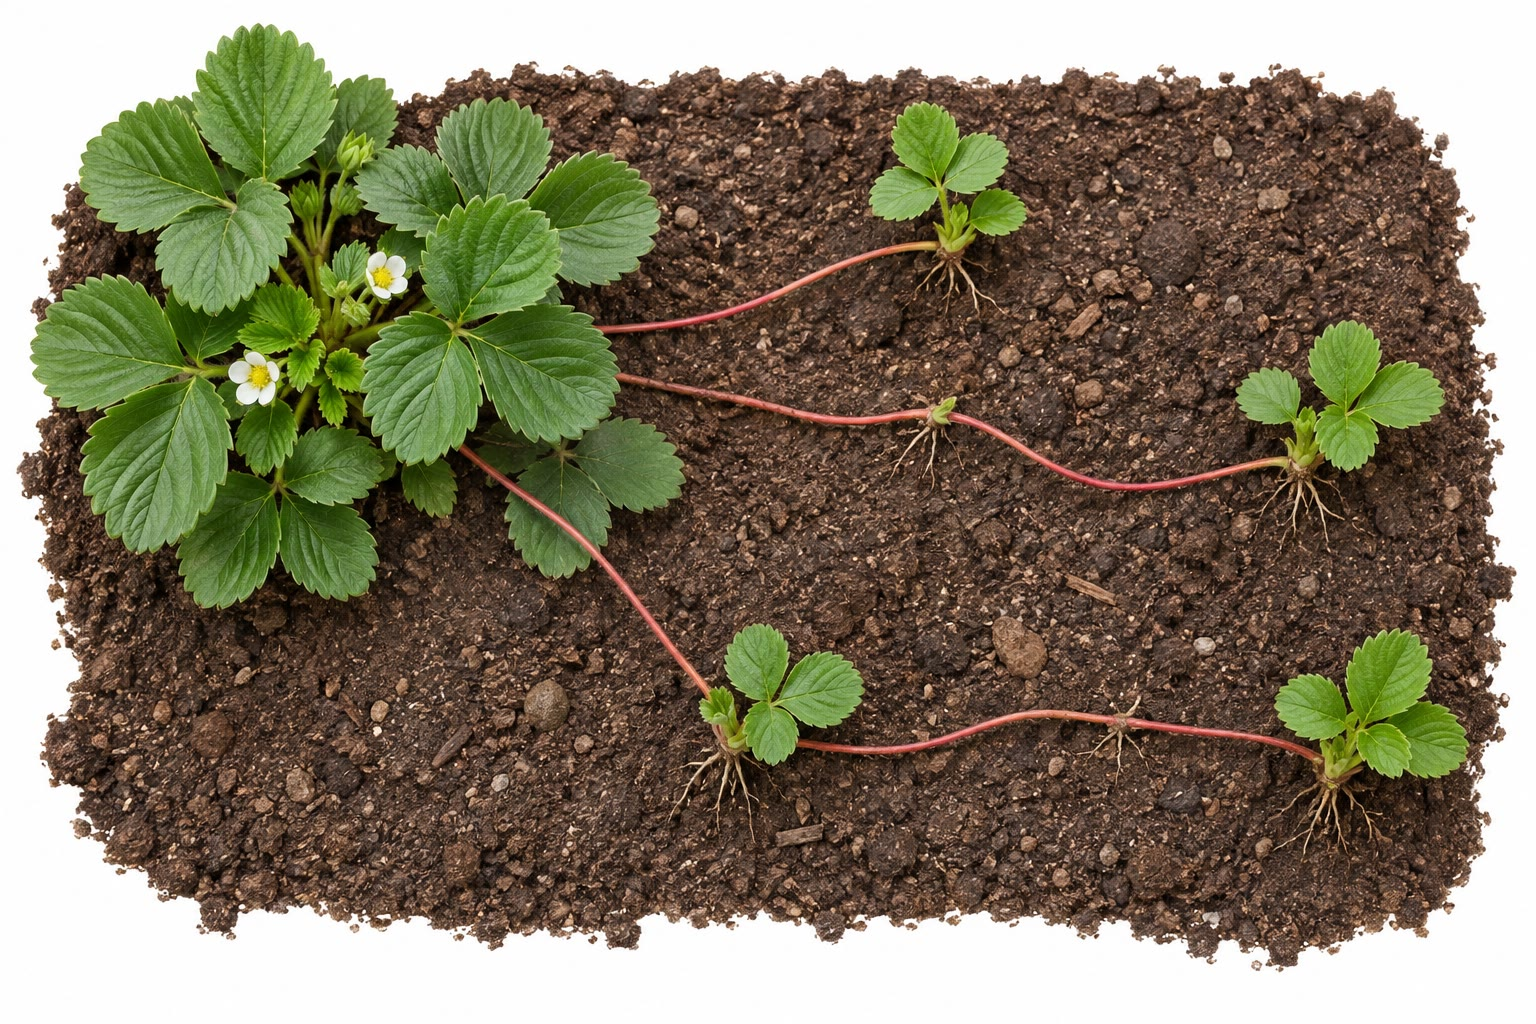
\includegraphics[width=0.46\linewidth]{images/book4/ai/b4-07-strawberry-runners.jpg}\hspace{0.03\linewidth}
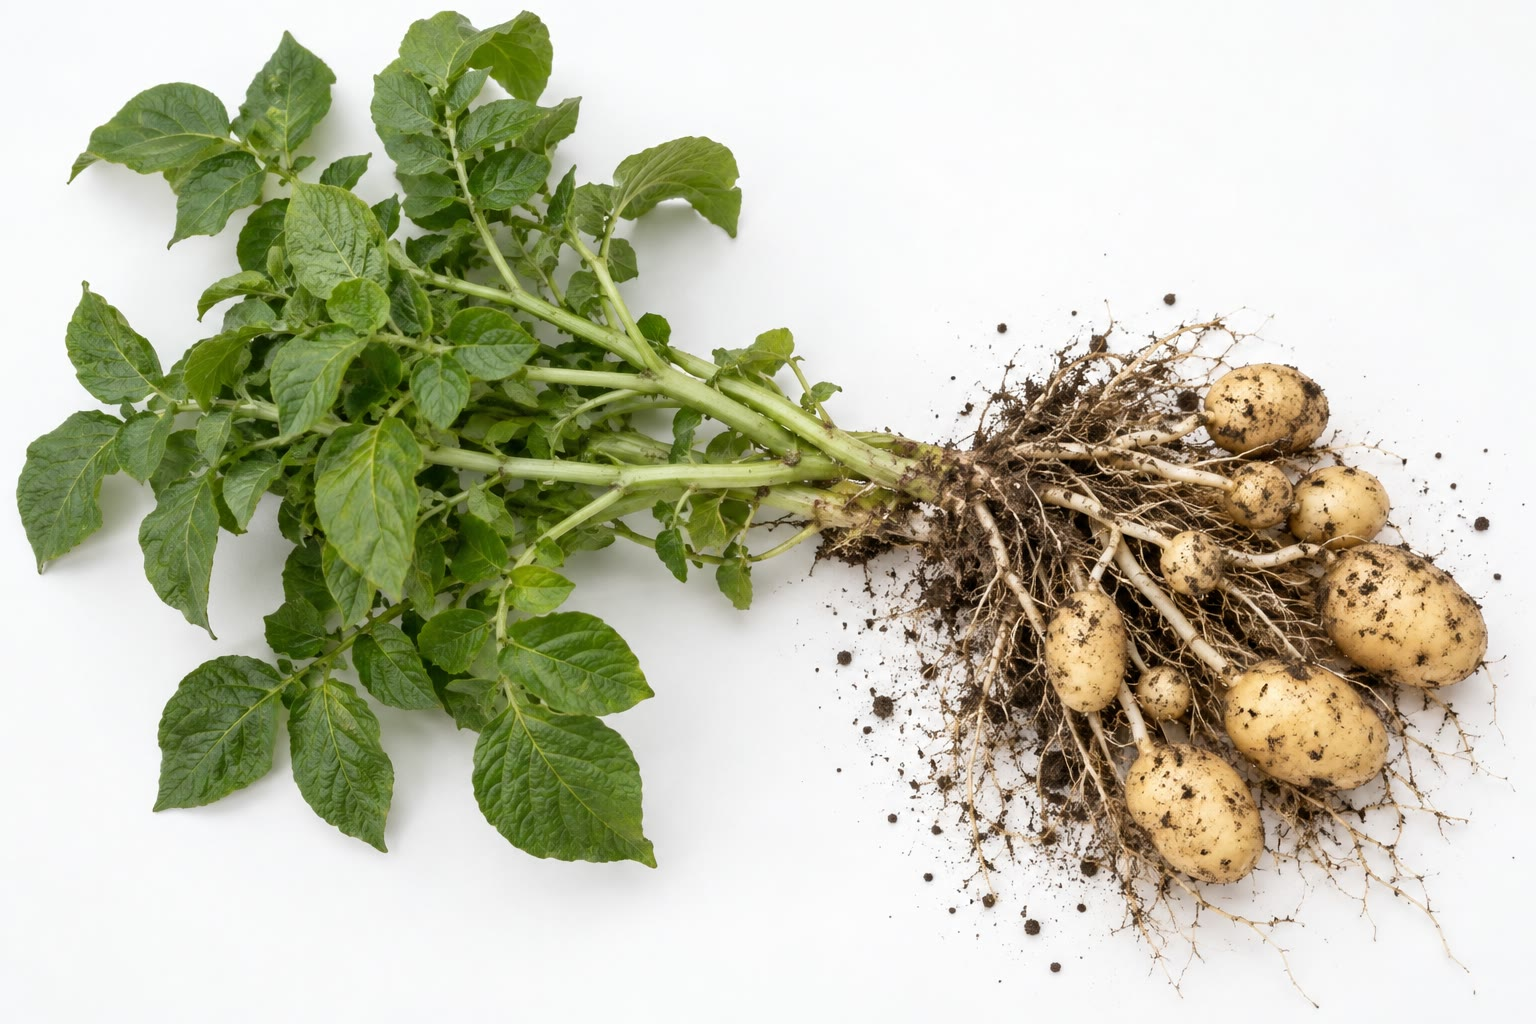
\includegraphics[width=0.46\linewidth]{images/book4/ai/b4-07-potato-tubers.jpg}

{\small 左：草莓植株及沿匍匐茎生根的子植株。
右：从土壤中挖出的马铃薯植株，其
\omterm{prop:b2:asexual-reproduction:organs}{块茎}悬挂于匍匐茎之上——每个\omterm{prop:b2:asexual-reproduction:organs}{块茎}都是一段茎，
将长成与之在遗传上完全相同的植株。}
\end{omfigure}

\begin{theorem}[扩展克隆的几何]\label{thm:b2:asexual-reproduction:spread}
\index{克隆生长}
若一个\omterm{def:b2:asexual-reproduction:clone}{基株}的每个\omterm{def:b2:asexual-reproduction:clone}{分株}每年产生 $m$ 个带根的子代，且全部存活，
则其数量按 $N(t) = N_0 (1 + m)^t$ 增长——
即在无任何有性过程的情况下呈指数增长——直至\omterm{def:b2:asexual-reproduction:clone}{分株}以其
环境容纳密度 $d$（单位面积上的\omterm{def:b2:asexual-reproduction:clone}{分株}数）充满空间，此后\omterm{def:b2:asexual-reproduction:clone}{克隆}
以前沿的形式推进。若一个\omterm{def:b2:asexual-reproduction:clone}{克隆}沿直线方向伸展其匍匐茎，
以速度 $v$ 推进，则经过 $t$ 年后，其半径为 $vt$，\omterm{def:b2:asexual-reproduction:clone}{分株}数
按 $\pi d (vt)^2$ 增长：呈二次方增长，而非指数增长。
一株每年伸出 \qty{0.5}{m} 匍匐茎的草莓植株，十年后
半径为 \qty{5}{m}；开篇提到的白杨\omterm{def:b2:asexual-reproduction:clone}{克隆}，
开篇段落中的白杨\omterm{def:b2:asexual-reproduction:clone}{克隆}，面积 \qty{43}{ha}，半径约 \qty{370}{m}，若以每年净推进几厘米计，其
年龄约为 $10^{4}$ 年——与
由冰川退缩估算的年龄相符。
\end{theorem}
\begin{proof}
每年，每个\omterm{def:b2:asexual-reproduction:clone}{分株}被其自身加 $m$ 个子代所取代，
因子为 $1 + m$；经过 $t$ 年得 $(1 + m)^t$。一旦内部
被充满，只有边缘的\omterm{def:b2:asexual-reproduction:clone}{分株}才有空间，边缘以
匍匐茎速度 $v$ 推进；面积为 $\pi(vt)^2$，\omterm{def:b2:asexual-reproduction:clone}{分株}数
即面积乘以密度。
\end{proof}

\begin{example}[最古老的生物]\label{ex:b2:asexual-reproduction:oldest}
白杨\omterm{def:b2:asexual-reproduction:clone}{克隆}体潘多（犹他州）覆盖 \qty{43}{ha}，约有
\num{47000} 根树干，每根约存活一个世纪，并被
同一根系长出的萌蘖取代；\omterm{def:b2:asexual-reproduction:clone}{基株}可能已超过一万
年。地中海的海草 \emph{Posidonia} \omterm{def:b2:asexual-reproduction:clone}{克隆}体
延伸 \qty{15}{km}，可能已有十万
年；莫哈韦沙漠中的煤焦油灌木环经测定为
\num{11700} 年，中心的茎随环扩展而死亡。在
每种情况下，老的是\omterm{def:b2:asexual-reproduction:clone}{基株}本身；其中没有任何细胞
的年龄超过几十年，而其基因组已被复制数千次。
\end{example}

\section{无性的种子与无父的动物}

\begin{definition}[无融合生殖]\label{def:b2:asexual-reproduction:apomixis}
\index{无融合生殖}\index{孤雌生殖}
\emph{无融合生殖}是指不经受精而产生\omterm{def:b2:angiosperm-reproduction:seed}{种子}：一个
胚由未经减数的卵细胞发育而来（\omterm{def:b2:plant-life-cycles:heterospory}{大孢子}母细胞
跳过\omterm{def:b2:meiosis-heredity:meiosis}{减数分裂}）或直接由珠心的一个细胞发育而来，且\omterm{def:b2:angiosperm-reproduction:seed}{种子}
携带母本的\omterm{def:b2:meiosis-heredity:vocabulary}{基因型}。蒲公英、山柳菊、黑莓、
肯塔基蓝草与许多柑橘都如此；柑橘\omterm{def:b2:angiosperm-reproduction:seed}{种子}常
含有数个胚，其中一个为有性胚，其余为母本
珠心的复制体。无融合生殖保留了\omterm{def:b2:angiosperm-reproduction:seed}{种子}——其扩散、\omterm{def:b2:angiosperm-reproduction:seed}{休眠}与\omterm{def:b2:angiosperm-reproduction:seed}{种皮}
——且省去\omterm{def:b2:meiosis-heredity:meiosis}{减数分裂}，使适应良好的\omterm{def:b2:meiosis-heredity:vocabulary}{基因型}
原样传播；多数无融合生殖植物为杂种起源的\omterm{def:b2:genome-diversification:polyploidy}{多倍体}，
其\omterm{def:b2:meiosis-heredity:meiosis}{减数分裂}本来就会失败。动物中与之对应的现象是
\emph{孤雌生殖}，即由未受精卵发育而来：
在某些蜥蜴与蛭形轮虫中为专性的，后者数千万年来
一直没有雄性；周期性的见于蚜虫与水蚤，
它们整个夏季进行孤雌生殖，雌体
直接产下已携带自身胚胎的活体雌性后代，并
在秋季转入有性世代，产下越冬
卵。
\end{definition}

\begin{omfigure}
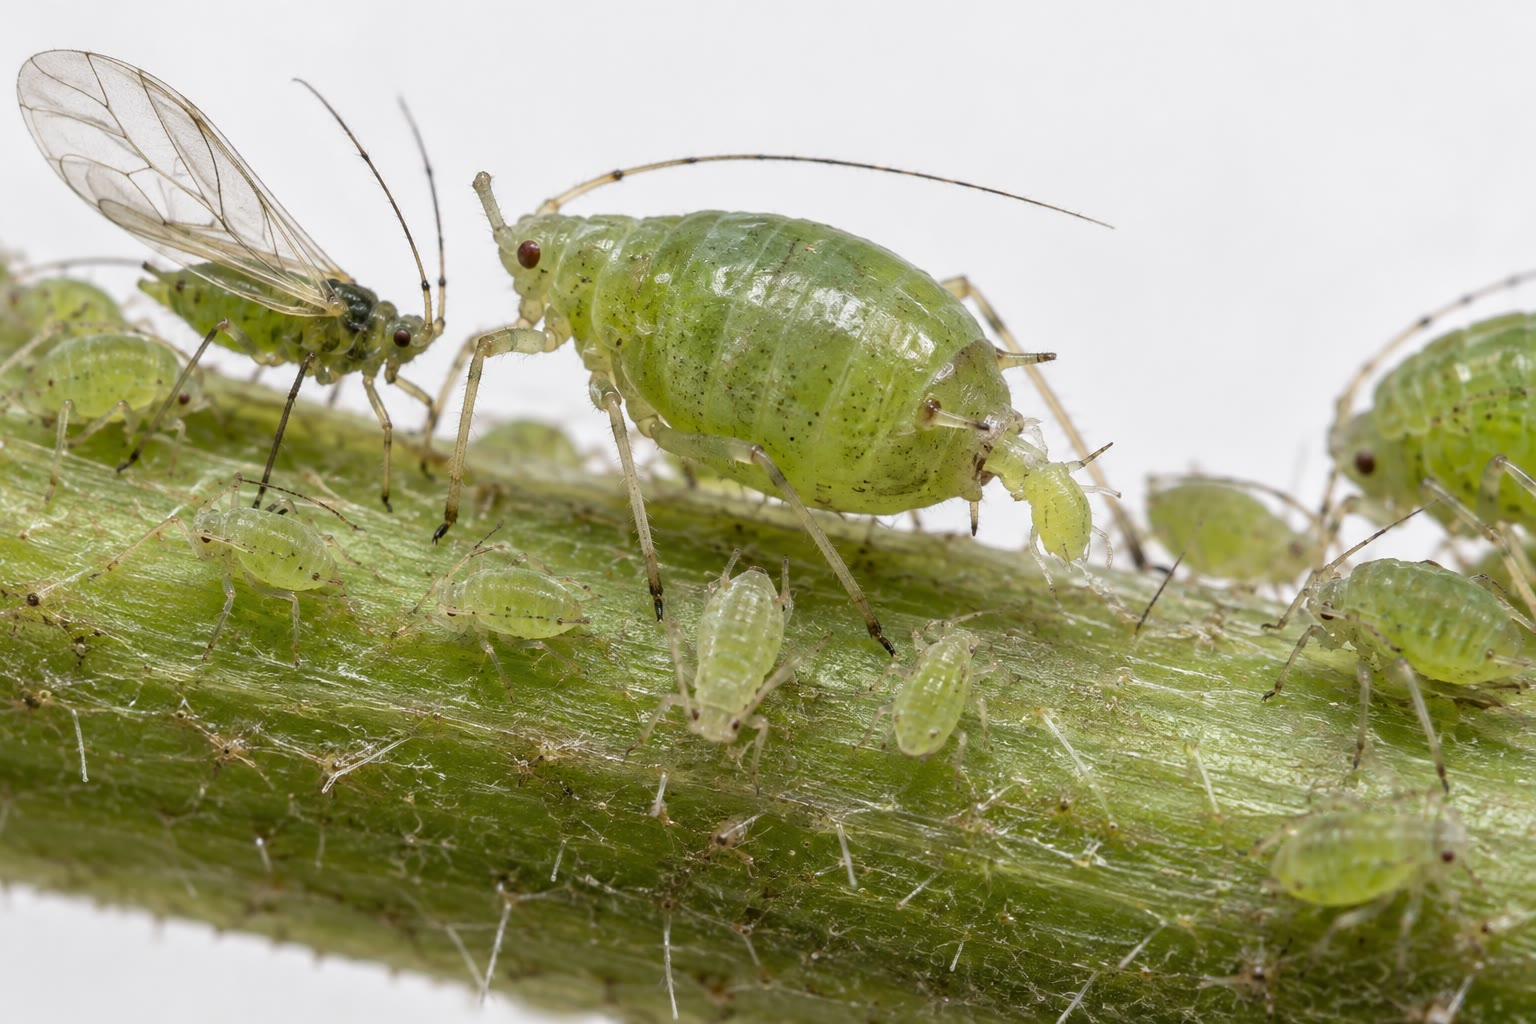
\includegraphics[width=0.55\linewidth]{images/book4/ai/b4-07-aphids.jpg}

{\small 茎上的蚜虫：一只无翅的\omterm{def:b2:asexual-reproduction:apomixis}{孤雌生殖}雌体，正在产下
一只活体雌性后代、多个龄期的若虫，以及一只有翅的
迁飞型个体——整个夏季的指数增长无需一只雄性。}
\end{omfigure}

\begin{example}[蚜虫的夏季]\label{ex:b2:asexual-reproduction:aphids}
一只\omterm{def:b2:asexual-reproduction:apomixis}{孤雌生殖}的蚜虫约八天成熟，随后两周内
每天产约五只雌性后代；这些后代出生时
即已怀孕（子代胚胎在母体的
胚胎内已开始发育）。\omterm{def:b2:unicellular-diversity:division}{世代时间}约十天，净增长率
约为每代 \num{50} 倍，若四月有一只始祖蚜虫
不受抑制，可留下 $50^{12} \approx 2\times 10^{20}$ 个后代，
四个月内——其总质量超过当今所有存活动物的总和。瓢虫、草蛉、
寄生蜂、真菌和降雨将数量控制在数千只
每株，秋季的有性世代将\omterm{def:b2:asexual-reproduction:clone}{克隆}重置为
冬前重组的卵。
\end{example}

\section{园艺栽培中的克隆}

\begin{proposition}[扦插、压条与嫁接]\label{prop:b2:asexual-reproduction:horticulture}
\index{扦插}\index{嫁接}\index{砧木}
\emph{\omterm{prop:b2:asexual-reproduction:horticulture}{扦插}}是指一段经诱导可生根的茎、根或叶：
切口端形成由分裂细胞构成的愈伤组织，由此长出根
分生组织，有赖于生长素（即生根激素）和湿度。
\emph{压条}是在枝条仍与母株相连时使其生根，然后
再切断。\emph{嫁接}是将一株植物的枝条（即
\emph{接穗}）接到另一株有根的茎（即\emph{\omterm{prop:b2:asexual-reproduction:horticulture}{砧木}}）上：
两者的形成层紧贴，愈伤组织弥合伤口，并
数周内新的木质部与韧皮部即跨越接口相连。嫁接体是一种
嵌合体——根保留\omterm{prop:b2:asexual-reproduction:horticulture}{砧木}的基因组，结果的枝条
保留接穗的基因组——嫁接只在亲缘相近的植物间才能成活（同属物种，
有时同科），因为两者的组织必须
能识别彼此的细胞。苹果、梨、樱桃、柑橘和
葡萄的每个品种都靠嫁接繁殖：一个有名称的品种即是一个
\omterm{def:b2:asexual-reproduction:clone}{基株}，借接穗存活数百年（雷内特苹果可追溯
到十六世纪），而\omterm{prop:b2:asexual-reproduction:horticulture}{砧木}的选择依据
土壤、病害和所需树形的大小——矮化
\omterm{prop:b2:asexual-reproduction:horticulture}{砧木}造就了现代果园中的小树。
\end{proposition}

\begin{proposition}[微繁殖与全能性]\label{prop:b2:asexual-reproduction:tissueculture}
\index{微繁殖}\index{全能性}\index{愈伤组织}
原则上，任何带细胞核的活植物细胞都能再生
出一株完整的植株。在\emph{组织培养}中，一块经灭菌的组织
（即\emph{外植体}：芽尖、叶盘或花药）被置于
含糖、无机盐、维生素和激素的琼脂培养基上。当
生长素与细胞分裂素比例适当时，细胞脱分化为
\emph{愈伤组织}，即由分裂中未特化细胞构成的团块；当
细胞分裂素多于生长素时，愈伤组织形成芽，生长素多于
细胞分裂素时形成根，某些物种中还形成\emph{体细胞
胚}——无需卵细胞的完整胚。
芽每隔数周切割并继代培养，每次扩增
三至十倍，因此一个分生组织在一
年内可得一百万株小植株。由于病毒滞后于生长点，芽分生组织
长度不足一毫米者，即使在受感染的
植株中，\emph{分生组织培养}正是马铃薯、草莓、香蕉和
兰花种苗得以净化。该方法是\omterm{prop:b2:asexual-reproduction:tissueculture}{全能性}的实际证明，
也是一个植物品种能在育成后数年内以
百万计售出的原因。
\end{proposition}
\begin{proof}[证据]
斯库格与米勒（1957）以烟草髓愈伤组织为材料，在
生长素与新发现的细胞分裂素比例不同的培养基上培养：高
生长素比例高则生根，细胞分裂素比例高则长芽，两者平衡则只
形成愈伤组织——器官的形成由两种激素的比例决定，而非
由某种特定的成器官物质决定。斯图尔德（1958）将
取自胡萝卜根的单细胞和小细胞团悬浮于旋转
培养瓶的椰乳中：一些细胞团形成了类胚结构，
它们发育成完整开花的胡萝卜，表明一个
成熟器官中已分化的细胞仍保有并能利用
整个发育程序。
\end{proof}

\begin{omfigure}
\begin{tikzpicture}[every node/.style={font=\scriptsize}, >=stealth]
  \node[draw, rounded corners, fill=omDef!12, align=center] (ex) at (0,0) {外植体 \\（茎尖、叶盘）};
  \node[draw, rounded corners, fill=omExo!30, align=center] (cal) at (4.6,0) {愈伤组织 \\生长素 $\approx$ 细胞分裂素};
  \node[draw, rounded corners, fill=omExo!30, align=center] (sh) at (8.4,1.2) {芽 \\细胞分裂素 $>$ 生长素};
  \node[draw, rounded corners, fill=omExo!30, align=center] (rt) at (8.4,-1.2) {根 \\生长素 $>$ 细胞分裂素};
  \node[draw, rounded corners, fill=omDef!12, align=center] (pl) at (12.2,0) {试管苗 \\在土壤中炼苗};
  \draw[->, thick] (ex) -- (cal) node[midway, below, align=center] {无菌 \\培养基};
  \draw[->, thick] (cal) -- (sh); \draw[->, thick] (cal) -- (rt);
  \draw[->, thick] (sh) -- (pl); \draw[->, thick] (rt) -- (pl);
  \draw[->, thick, omThm] (sh) .. controls (8.4,2.6) and (5.8,2.6) .. (5.2,0.6);
  \node[omThm, anchor=south] at (6.9,2.3) {每 4 周继代一次，$\times 5$};
\end{tikzpicture}

{\small \omterm{prop:b2:asexual-reproduction:tissueculture}{微繁殖}：外植体脱分化形成
愈伤组织，由生长素与细胞分裂素的比例引导形成芽或根，
再经反复继代培养增殖，然后将小植株
炼苗后移入土壤。}
\end{omfigure}

\begin{omfigure}
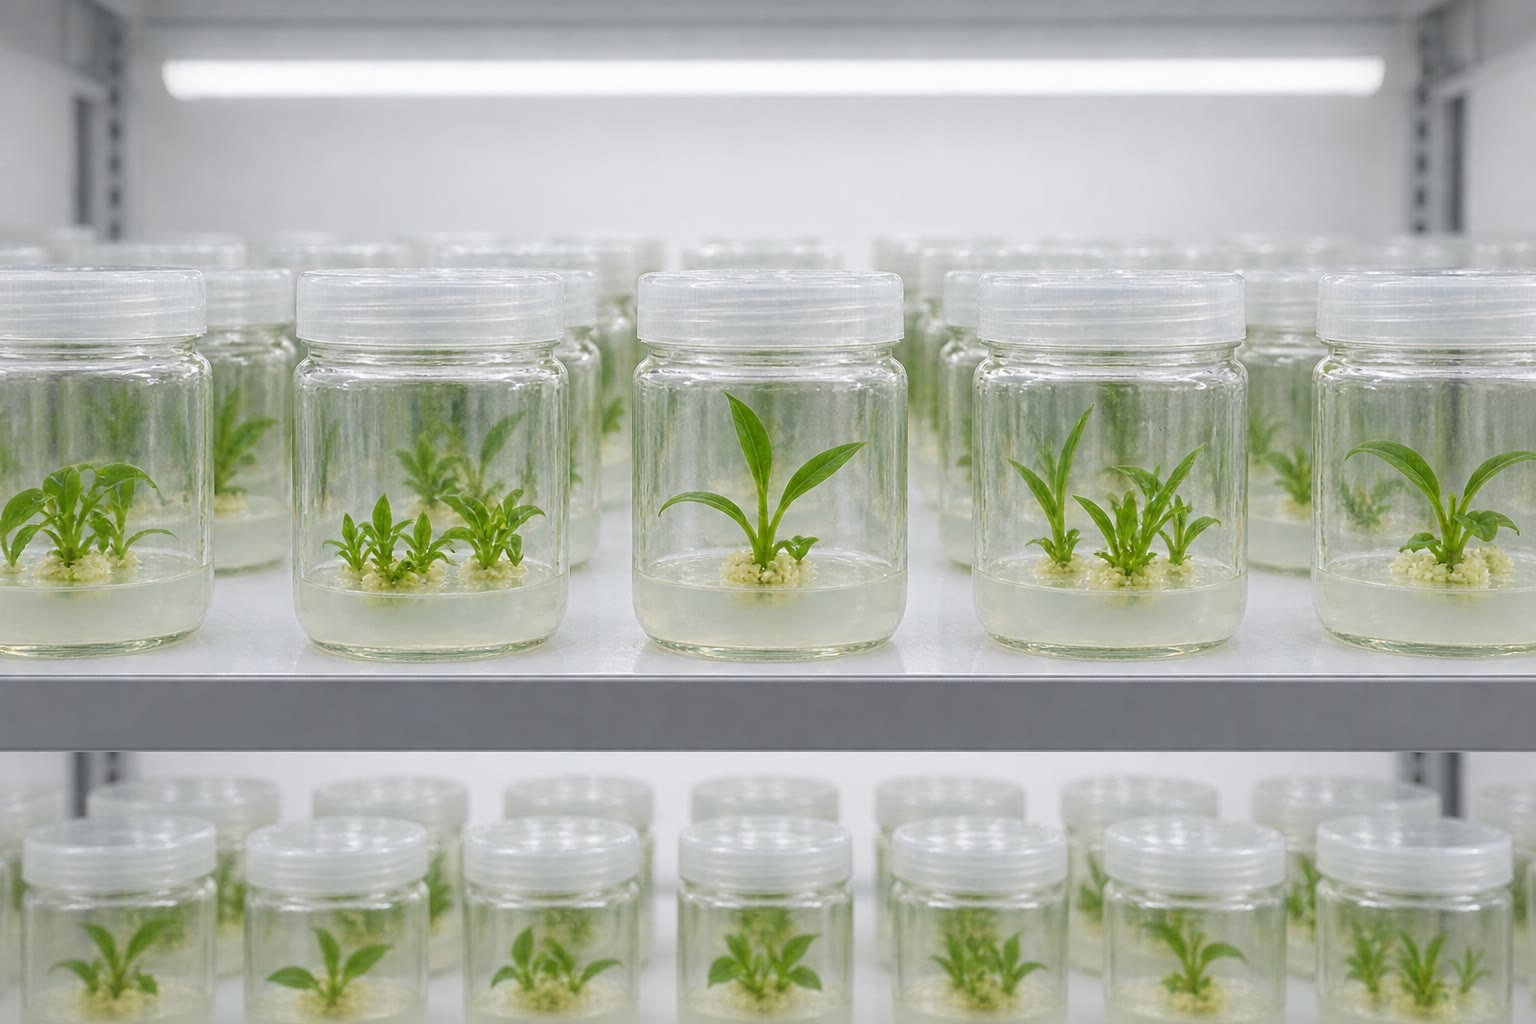
\includegraphics[width=0.6\linewidth]{images/book4/ai/b4-07-tissue-culture.jpg}

{\small 培养室中琼脂培养基上的试管苗：每个瓶中
所含植株均为同一品种的一个无性系，由单个分生组织增殖而来。}
\end{omfigure}

\section{有性生殖的代价与放弃有性生殖的代价}

\begin{theorem}[有性生殖的双倍代价]\label{thm:b2:asexual-reproduction:twofold}
\index{有性生殖的双倍代价}
在一个种群中，每个雌性产生 $F$ 个后代，其中一半
为雄性。一个无性\omterm{def:b2:genome-diversification:mutation}{突变}雌性产生 $F$ 个女儿，
全部为其自身的复本，使其在下一代雌性中
所占份额翻倍。若无性系在雌性中的频率为 $p$，
则下一代中
\[
p' = \frac{2p}{1 + p}, \qquad p_t = \frac{2^t p_0}{1 + (2^t - 1)p_0},
\]
于是从千分之一出发，无性系在
十代内即可达到种群的一半，此后很快占据全部。其他条件相同时，
有性生殖使谱系的增殖速率减半——即
产生雄性的代价。由于有性生殖仍几乎普遍存在，
说明其他条件并不相同：有性谱系平均而言必须通过重组
获得至少两倍的增益。
\end{theorem}
\begin{proof}
无性雌性数为 $pN$，产生 $FpN$ 个女儿；有性
雌性数为 $(1 - p)N$，产生 $F(1 - p)N/2$ 个女儿（
另一半为雄性，不产卵）。无性雌性在女儿中
所占份额为 $Fp/(Fp + F(1 - p)/2) = 2p/(1 + p)$。记 $q = p/(1 -
p)$，则递推式变为 $q' = 2q$，故 $q_t = 2^t q_0$；换回
即得 $p_t$。令 $p_t = \tfrac12$，得 $2^t q_0 = 1$，即\
$t = \log_2(1/q_0) \approx 10$（当 $p_0 = 10^{-3}$ 时）。
\end{proof}

\begin{omfigure}
\begin{tikzpicture}
\begin{axis}[
  width=0.76\linewidth, height=5.6cm,
  axis x line=bottom, axis y line=left,
  xmin=0, xmax=20, ymin=0, ymax=1.05,
  xlabel={世代}, ylabel={无性系的频率},
  xlabel style={font=\small, at={(axis description cs:0.5,-0.13)}, anchor=north},
  ylabel style={font=\small},
  tick label style={font=\small}, xtick={0,5,10,15,20}, ytick={0,0.5,1},
  legend style={font=\scriptsize, at={(0.5,-0.3)}, anchor=north, draw=none},
  clip=false,
]
\addplot[very thick, omThm, domain=0:20, samples=80] {2^x*0.001/(1+(2^x-1)*0.001)};
\addlegendentry{无其他差异：12 代内取代}
\addplot[very thick, omDef, domain=0:20, samples=80] {0.001*(1.3)^x/(1+(1.3^x-1)*0.001)};
\addlegendentry{无性系因寄生生物损失 \qty{35}{\%} 的适合度：增长较慢}
\addplot[very thick, omProp, domain=0:20, samples=80] {0.001*(0.9)^x/(1+(0.9^x-1)*0.001)};
\addlegendentry{无性系损失 \qty{55}{\%}：永不扩散}
\end{axis}
\end{tikzpicture}

{\small 双倍优势的实际效果。从千分之一起始，
无其他劣势的无性系
约 12 代内即可取代种群；只有至少一半的适合度损失
——来自寄生生物、累积\omterm{def:b2:genome-diversification:mutation}{突变}或适应变慢——
才能将其遏制。}
\end{omfigure}

\begin{proposition}[有性生殖的作用]\label{prop:b2:asexual-reproduction:whysex}
\index{穆勒棘轮}\index{红皇后假说}
三种好处足够重要。\emph{\omterm{prop:b2:asexual-reproduction:whysex}{穆勒棘轮}}：
在一个\omterm{def:b2:asexual-reproduction:clone}{克隆}中，每个有害\omterm{def:b2:genome-diversification:mutation}{突变}都遗传给所有后代，
而无\omterm{def:b2:genome-diversification:mutation}{突变}的基因组一旦因偶然而从有限种群中丢失，
便永远无法重建；遗传负荷如棘轮般逐步上升，
每次一格，小型无性种群因此衰退。重组可由
两个受损的基因组重建洁净基因组。\emph{适应}：两个有益\omterm{def:b2:genome-diversification:mutation}{突变}
若出现在同一\omterm{def:b2:asexual-reproduction:clone}{克隆}的不同个体中，则相互竞争，
其中一个丢失；在有性种群中二者可以结合（费希尔与穆勒，
1930 年代），因此当许多基因必须发生改变时，
有性种群适应更快。\emph{红皇后}：寄生生物适应最常见的宿主
\omterm{def:b2:meiosis-heredity:vocabulary}{基因型}，而\omterm{def:b2:asexual-reproduction:clone}{克隆}本身即是单一\omterm{def:b2:meiosis-heredity:vocabulary}{基因型}，因而最为常见；
有性亲本使每个后代都成为一把新的“锁”。蜗牛、鱼类和
植物，若同时具有有性种群与\omterm{def:b2:asexual-reproduction:clone}{克隆}种群，则显示
有性种群在寄生生物丰富处占优势。繁盛的无性
谱系——蒲公英、蛭形轮虫、多数作物
\omterm{def:b2:asexual-reproduction:clone}{克隆}——要么年轻，要么是携带自身变异的\omterm{def:b2:genome-diversification:polyploidy}{多倍体}杂种，
或靠种植者扶持而存续，种植者代其
杀灭寄生生物。
\end{proposition}

\begin{example}[同一克隆的单一栽培]\label{ex:b2:asexual-reproduction:monoculture}
1840 年代，爱尔兰马铃薯作物大部分为同一无性系品种，
即 Lumper；卵菌 \emph{Phytophthora infestans}，
1845 年传入，所遇之地布满基因相同、
普遍易感的植株，连续三年摧毁了作物。
1950 年代以前，世界出口的香蕉是单一\omterm{def:b2:asexual-reproduction:clone}{克隆}，即大米
歇尔，后在中美洲种植园被土壤真菌摧毁；
其替代品卡文迪什同样是单一\omterm{def:b2:asexual-reproduction:clone}{克隆}，目前
正逐个种植园地被同一真菌的新菌株侵袭，
而它没有可供抵抗的变异。\omterm{def:b2:asexual-reproduction:clone}{克隆}是
自然界中最容易受攻击的目标，种植\omterm{def:b2:asexual-reproduction:clone}{克隆}的人必须提供
重组本可免费提供的抗性。
\end{example}

\section{练习}

\begin{exercise}[$\star$]\label{exo:b2:asexual-reproduction:1}
定义\omterm{def:b2:asexual-reproduction:clone}{克隆}、\omterm{def:b2:asexual-reproduction:clone}{基株}和\omterm{def:b2:asexual-reproduction:clone}{分株}，并为每种植物列出
三种天然的\omterm{def:b2:asexual-reproduction:clone}{营养增殖}器官。
\end{exercise}

\begin{exercise}[$\star$]\label{exo:b2:asexual-reproduction:2}
在嫁接中，要使接口愈合成功，两部分的哪些组织必须相接，
\omterm{prop:b2:asexual-reproduction:horticulture}{砧木}与接穗各自为树体贡献什么？
为何嫁接树是嵌合体而不是杂种？
\end{exercise}

\begin{exercise}[$\star$]\label{exo:b2:asexual-reproduction:3}
区分\omterm{def:b2:asexual-reproduction:apomixis}{无融合生殖}与\omterm{def:b2:asexual-reproduction:clone}{营养增殖}，
并区分\omterm{def:b2:asexual-reproduction:apomixis}{孤雌生殖}与这两者。三者中哪一种保留\omterm{def:b2:angiosperm-reproduction:seed}{种子}？
\end{exercise}

\begin{exercise}[$\star$]\label{exo:b2:asexual-reproduction:4}
列出\omterm{prop:b2:asexual-reproduction:tissueculture}{微繁殖}从外植体到田间植株的各步骤，
并说明每一步的激素条件。
\end{exercise}

\begin{exercise}[$\star\star$]\label{exo:b2:asexual-reproduction:5}
一株草莓每年长出 8 条匍匐茎，每条匍匐茎生根
形成 3 株小植株，每株小植株次年重复同样的过程。
若无植株死亡，4 年后共有多少株？每株按 \qty{0.1}{m^2} 计，
它们需要多大面积？究竟是什么限制了这一\omterm{def:b2:asexual-reproduction:clone}{克隆}的增长？
\end{exercise}

\begin{exercise}[$\star\star$]\label{exo:b2:asexual-reproduction:6}
颤杨\omterm{def:b2:asexual-reproduction:clone}{克隆} Pando 在 \qty{43}{ha} 上有 \num{47000} 根树干，
每根树干约存活 \num{130} 年。若\omterm{def:b2:asexual-reproduction:clone}{基株}年龄为 \num{14000} 年，
它历经了多少代树干？计算其平均径向扩展速度，
单位为米每年，并将其视为圆盘。
\end{exercise}

\begin{exercise}[$\star\star$]\label{exo:b2:asexual-reproduction:7}
在一个有性种群中，一个无性\omterm{def:b2:genome-diversification:mutation}{突变}体以频率 $10^{-4}$ 出现，
两者繁殖力相同。计算其经过 5、
10 和 15 代后的频率。它的适合度须降低多少，
才能使其永不扩散？
\end{exercise}

\begin{exercise}[$\star\star$]\label{exo:b2:asexual-reproduction:8}
预测烟草愈伤组织在生长素：细胞分裂素
比例为 10 : 1、1 : 1 和 1 : 10 的培养基上将如何生长，并解释
为何嫩枝插条应浸于生长素而非细胞分裂素中。
\end{exercise}

\begin{exercise}[$\star\star$]\label{exo:b2:asexual-reproduction:9}
马铃薯以\omterm{prop:b2:asexual-reproduction:organs}{块茎}种植。每种植一千克，可收获
\qty{10}{kg}，一公顷需要 \qty{2}{t} 种薯。以
\qty{1}{kg} 的新品种为起点，需要几个季节才能
种满一公顷？为何真\omterm{def:b2:angiosperm-reproduction:seed}{种子}的繁殖更快，却
不被采用？
\end{exercise}

\begin{exercise}[$\star\star\star$]\label{exo:b2:asexual-reproduction:10}
在含 $N$ 个个体的\omterm{def:b2:asexual-reproduction:clone}{克隆}种群中，每个基因组每代
产生 $U$ 个有害\omterm{def:b2:genome-diversification:mutation}{突变}，每个\omterm{def:b2:genome-diversification:mutation}{突变}使适合度损失比例 $s$，
则平衡时无\omterm{def:b2:genome-diversification:mutation}{突变}个体所占比例为
$e^{-U/s}$（推导见\cref{ch:b2:population-genetics}）。取 $U =
0.1$ 与 $s = 0.02$，计算
当 $N = 10^{5}$ 与 $N = 10^{3}$ 时无\omterm{def:b2:genome-diversification:mutation}{突变}个体的数目，并结合
\omterm{prop:b2:asexual-reproduction:whysex}{穆勒棘轮}，解释为何小种群注定灭绝，而大种群
则尚未如此——但未必永远如此。
\end{exercise}

\begin{exercise}[$\star\star\star$]\label{exo:b2:asexual-reproduction:11}
一种能克服某一\omterm{def:b2:meiosis-heredity:vocabulary}{基因型}抗性的病原体菌株
仅出现一次。比较它在单一\omterm{def:b2:asexual-reproduction:clone}{克隆}田间与
有性种群中的命运，其中抗性基因在十个位点上分离，
每个位点有两个\omterm{def:b2:meiosis-heredity:vocabulary}{等位基因}且频率相等，并用这些概念解释爱尔兰
马铃薯饥荒。
\end{exercise}

\begin{exercise}[$\star\star\star$]\label{exo:b2:asexual-reproduction:12}
“有性繁殖代价为两倍，却处处可见；无性繁殖廉价而
罕见。”讨论本章的三种解释，并说明
蛭形轮虫——已无性繁殖四千万年——对
每种解释有何启示。
\end{exercise}

\section{问题：草莓农场与一个古老的克隆}

\begin{problem}[{周末问题——克隆的算术，从由匍匐茎铺满的草莓田，
到实验室增殖一个分生组织，
到无融合生殖者入侵有性种群，
再到一个古老基株的遗传衰变，最后归结为铺满田地所需的时间、
由一个分生组织得到的小植株数，
以及无融合生殖者与有性个体的平衡}]
\label{pb:b2:asexual-reproduction:1}
一位种植者在一块田地上种下 \num{100} 株草莓，
这块 \qty{1}{ha} 的田地每平方米可容纳 \num{4} 株。每株
一年可长出 \num{6} 条匍匐茎，每条匍匐茎生根形成 \num{2} 株子株，
所有植株均存活。一间实验室以组织培养繁殖同一品种：
组织培养中，每次继代（每 \num{4} 周一次）使芽数
扩增 \num{5} 倍；\qty{80}{\%} 的小植株可在炼苗后存活。
该品种的普通\omterm{prop:b2:asexual-reproduction:horticulture}{扦插}枝条有 \qty{90}{\%} 带病毒；
\qty{0.3}{mm} 的分生组织顶端携带病毒的概率为
$0.02$。颤杨基因组：\qty{4.8e8}{} 碱基对；体细胞\omterm{def:b2:genome-diversification:mutation}{突变}率
\qty{1e-9}{}（每碱基对每次细胞分裂）；生长中的芽的分生组织细胞
每年分裂 \num{20} 次。

\medskip
\noindent\textbf{第一部分——铺满田地。}
\begin{enumerate}
  \item 这块田地最多可容纳多少株？
  \item 植株数量每年按什么倍数增长？
  \item 计算 1、2 和 3 年后的植株数。
  \item 解方程 $N(t) = 100\times 13^{t}$，求
        田地铺满的时刻。
  \item 田地铺满后，只有斑块边缘的植株
        还能找到空间。若斑块每年扩展 \qty{0.5}{m}，则一株
        仅靠扩展需要多少年才能覆盖整块田地？
  \item 解释种植者为何将 \num{100} 株植株分散
        布满整块田地，而不是只种一株。
\end{enumerate}

\medskip
\noindent\textbf{第二部分——实验室。}
\begin{enumerate}[resume]
  \item 从一个分生组织出发，需要多少次继代培养，
        才能得到至少 $10^{6}$ 个芽？需要多少周？
  \item 有多少株植株能在驯化过程中存活？
  \item 由分生组织得到的株系无病毒的概率是多少？
        由同一株植物开始的 \num{10} 个株系全部
        无病毒的概率又是多少？
  \item 实验室启动 \num{10} 个株系，并在检测后剔除感染株系。
        期望的无病毒株系数是多少？并与
        \omterm{prop:b2:asexual-reproduction:horticulture}{扦插}法进行比较。
  \item 解释分生组织顶端为何能避开病毒。
  \item 田地可以在第一年直接由实验室的产出种植，
        而不必像靠匍匐茎那样用三年时间铺满。
        请分别给出两种途径各一个优点和一个风险。
\end{enumerate}

\medskip
\noindent\textbf{第三部分——\omterm{def:b2:asexual-reproduction:apomixis}{无融合生殖}个体入侵。}
蒲公英种群为有性生殖。一种\omterm{def:b2:asexual-reproduction:apomixis}{无融合生殖}（\omterm{def:b2:angiosperm-reproduction:seed}{种子}\omterm{def:b2:asexual-reproduction:clone}{克隆}）\omterm{def:b2:genome-diversification:mutation}{突变}体
以频率 $p_0 = 10^{-3}$ 出现，其每株\omterm{def:b2:angiosperm-reproduction:seed}{种子}产量与
有性植株相同。有性植株一半的繁殖投入
用于\omterm{def:b2:plant-life-cycles:heterospory}{花粉}。
\begin{enumerate}[resume]
  \item 论证\omterm{def:b2:asexual-reproduction:apomixis}{无融合生殖}个体在\omterm{def:b2:angiosperm-reproduction:seed}{种子}亲本中频率的
        递推式 $p' = 2p/(1 + p)$ 的合理性。
  \item 计算 5 代和 10 代后的 $p$，并求
        频率超过一半时所在的世代。
  \item 一种锈菌专门寄生于最常见的\omterm{def:b2:meiosis-heredity:vocabulary}{基因型}：\omterm{def:b2:asexual-reproduction:apomixis}{无融合生殖}个体的\omterm{def:b2:angiosperm-reproduction:seed}{种子}产量
        被乘以因子 $(1 - cp)$，其中
        $c = 0.8$。写出新的递推式。
  \item 求平衡频率 $p^*$，并由 $p' - p$ 的符号
        判断其两侧的稳定性。
  \item 当 $c$ 取何值时，\omterm{def:b2:asexual-reproduction:apomixis}{无融合生殖}个体会完全取代有性个体？
  \item 计算 $c = 0.6$ 时的平衡频率，并加以解释：
        寄生生物必须做什么，才能保护有性生殖？
  \item \omterm{def:b2:asexual-reproduction:apomixis}{无融合生殖}个体是三倍体。为何它不能回到有性生殖，
        这一点从长远看为何重要？
\end{enumerate}

\medskip
\noindent\textbf{第四部分——古老的\omterm{def:b2:asexual-reproduction:clone}{克隆}。}
\begin{enumerate}[resume]
  \item 计算颤杨中每次细胞分裂
        所产生的体细胞\omterm{def:b2:genome-diversification:mutation}{突变}数。
  \item Pando \omterm{def:b2:asexual-reproduction:clone}{克隆}的两个树干在共同祖先两侧各生长了 \num{14000}
        年。它们之间相隔多少次细胞分裂，以及
        有多少个\omterm{def:b2:genome-diversification:mutation}{突变}使其基因组
        相互区别？
  \item 这占基因组的比例是多少？若基因组的 \qty{2}{\%}
        为编码区，则有多少个编码差异？
  \item \omterm{def:b2:asexual-reproduction:clone}{克隆}个体不进行\omterm{def:b2:meiosis-heredity:meiosis}{减数分裂}，在个体水平上也没有选择
        能够清除这些\omterm{def:b2:genome-diversification:mutation}{突变}。那么，是什么清除了它们，
        以及为何这种“筛选”比在有性谱系中更弱？
  \item Pando 是否“遗传上一致”？请用两句话讨论。
  \item 给出结果：匍匐茎铺满田地所需的时间、一个分生组织
        一年内产生的小植株数，以及\omterm{def:b2:asexual-reproduction:apomixis}{无融合生殖}个体在
        $c = 0.8$ 时的平衡频率。
\end{enumerate}
\end{problem}
